\section{Transmisión de datos en banda ancha}
La banda ancha surge de la necesidad de cambiar la utilidad de las redes clásicas, es decir, adaptarse a las nuevas necesidades. Ahora las redes se usan más para la transmisión de datos que de voz.\\
Las redes se dividirán en:
\begin{itemize}
\item Red de acceso, conecta al usuario con la red.
\item Red troncal, secciones internas de las grandes redes de los proveedores de internet(\acrshort{ISP}).
\end{itemize}
Al principio se optó por opciones como la Jerarquía Digital Plexincrona (\acrshort{PDH}). Los sistemas MIC agrupan canales de 64kbps. El sistema MIC de norma europea agrupa 30 canales produciendo 2Mbps de transmisión y el americano 24 canales produciendo 1.5Mbps de transmisión.
\subsection{\acrshort{RDSI}}
La Red Digital de Servicios Integrados(\acrshort{RDSI}) es la siguiente evolución y ofrece dos canales por terminalque se podrán utilizar de la forma que cada uno decida. Este sistema tiene un latencia muy baja que aún no se ha podido igualar. Se utiliza \acrshort{TDM} con un envío de un paquete de 8 bits cada 125 microsegundos.
\subsubsection{Estructura \acrshort{RDSI}}
Como se puede ver en la imagen la estructura del \acrshort{RDSI} es muy simple. La sección del \acrshort{ISP} termina en TR1 que es la roseta de entrada a casa.
\begin{figure}[htp]
	\centering
	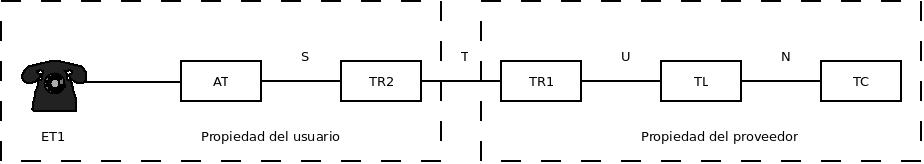
\includegraphics[width=\textwidth]{Imagen/diaRDSI.jpg}
	\caption{Estructura del sistema \acrshort{RDSI}}
	\label{}
\end{figure}
Las difierentes piezas de la estructura son:
\begin{itemize}
	\item ET1: estación terminal. Con acceso básico podrían colocarse 2 terminales. estos son ordenadores, telefonos, etc.
	\item AT: este módulo se utiliza para adaptar telefonos analógicos al sistema digital. Este no siempre es necesario.
	\item TR2: una centralita de distribución, separa los canales para los diferentes terminales. No siempre hay uno
	\item TR1: roseta de entrada. Primer elemento perteneciente al ISP.
	\item TL y TC: son parte de la central local.
\end{itemize}
Las interfaces que conectan los anteriores son:
\begin{itemize}
	\item Interfaz S: 192kbps
	\item Interfaz T
	\item Interfaz U: 160kbps en acceso básico y 2mbps (europa), 1.5mbps (américa) en acceso primario.
	\item Interfaz N
\end{itemize}
Las interfaces S y T presentan la peculiaridad de ser iguales electricamente, es decir en caso de que no halla un TR2 la estación terminal se puede conctar directamente a la roseta. Esto no quita que en caso necesario las modulaciones o accesos multiples se puedan diferenciar.\\
\subsubsection{Accesos}
Los diferentes accesos se configuran en función de la configuración de diferentes canales.
\begin{itemize}
	\item Canal B: Transmite infromación a una velocidad de 64kbps.
	\item Canal D: Es un canal de señalización que va entre 16 y 64 kbps.
	\item Canal H: Transmite información a una velocidad superior a 64kbps.
\end{itemize}
Un acceso básico incluye dos canales B y un canal D (a 16kbps). Un acceso primario coincide con los sistemas MIC del sistema \acrshort{PDH}. El acceso primario se constituye de 30 canales B y un canal D (a 64kbps) en europa y 23 canales B en américa.
\subsection{Banda ancha en núcleo de abonado xDSL}
Utilización del bucle de abonado más allá del telefono. Hace uso de modulaciones multiportadora adaptada. Se analiza el canal y se diseña en que frecuencias se utilizan que modulaciones para utilizar mejor el ancho de banda. En algunos casos por la cercania entre bandas es necesaria la utilización de cancelación de ecos.
\subsection{\acrshort{SDH}}
Conjunto jerárquico de estructuras digitales de transporte de cargas adaptadas sobre redes de transmisión física". Se trata de una técnica de multiplexación utilizada normalmente en los sistemas de fibra óptica. Ha sido adaptado también a sistemas de cable coaxial.\\
El \acrshort{SDH} utiliza como unidad básica el \acrshort{STM}-1 (Módulo de Transferencia Sincrona). en la figura se puede ver la estructura lógica de un \acrshort{STM}-1.
\begin{figure}[H]
\centering
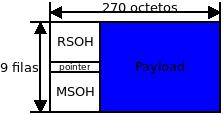
\includegraphics[width=0.7\textwidth]{Imagen/diaSTM1.jpg}
\caption{Estructura lógica de la trama STM-1}
\end{figure}
\begin{itemize}
	\item Payload: Donde se guardan los datos enviados por los usuarios.
	\item RSOH: Cabezera de regeneración (al ser fibra hey que regenerar la señal cada poco espacio. CRC's, etc.
	\item MSOH: Cabezera de multiplexación, número de cargas, posición de cada una de ellas, etc.
	\item Pointer: Puntero al inicio de la carga util.
\end{itemize}
\subsubsection{Estructura de la multiplexación en \acrshort{SDH}}
En la siguiente figura se puede ver la estructura seguida para la multiplexación de los diferentes contenedores de carga.
\begin{figure}[H]
\centering
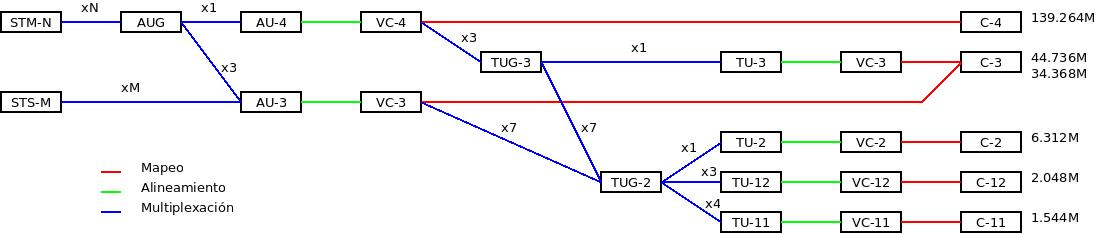
\includegraphics[width=\textwidth]{Imagen/diamuxSDH.jpg}
\caption{Estructura de la multiplexación en \acrshort{SDH}}
\end{figure}
\begin{itemize}
	\item C-x: Contenedor número x. Espacio de la trama dedicado a datos, se mide en Mbps. Un C-4 ocupa todo el espacio de payload de un STM-1.
	\item VC-x: Contenedor Virtual es un C-x con información del contenido del mismo. POH+C-x=VC-x
	\item AU-x: Unidad administrativa. Incluye un puntero a los contenedores virtuales
	\item TU-x: Unidad Tributaria, incluye información de la tarificación.
	\item TUG-x: Unidad Tributaria y de Gestión.
	\item AUG: Unidad Administrativa y de gestión.
	\item STS: es la unidad básica de la adaptación de SDH para el cable coaxial, similar al STM para la fibra óptica.
	\item STM: Módulo de Transferencia Síncrona.
\end{itemize}
El acto de mapear se da en el paso de un contenedor a su contenedor virtual. El alineamiento de los diferentes contenedores virtuales se produce para la obtención de unidades administrativas y tributarias. La multiplexación se produce al juntar todos los sistemas menores dentro de los \acrshort{STM}.\\
Dentro de un \acrshort{STM}-1 se pueden contener los siguientes contenedores:
\[STM-1=
\begin{cases}
63, & \text{c-12}\\
21, & \text{c-2}\\
3, & \text{c-3}\\
1, & \text{c-4}
\end{cases}
\]
\subsubsection{\acrshort{SNCP} SubNetwork Connection Protection}
En fibra óptica siempre se encuentran pares de fibra ya que los componentes no son recíprocos. El emisor solo es capaz de transmitir y el receptor solo puede recibir. Además los sistemas de fibra siempre toman forma de anillo, en caso de ruptura.\\
\acrshort{SNCP} es un sistema similar a flooding. Todos los paquetes se envian por ambos lados del anillo. El mayor problema es que reduce a la mitad la capacidad de los enlaces. En cambio todos los nodos reciben información sobre los enlaces caidos.
\subsubsection{MS-Spring}
Este sistema de protección está diseñado para sistemas STM-16 en adelante. A diferencia de \acrshort{SNCP} el anillo tiene la capacidad completa hasta que alguno de los nodos se rompe. En caso de caida, la capacidad se divide a la mitad. Este sistema protege a nivel de contenedor virtual 4. \\
Si se elige dar prioridad a la protección se descartarán cargas utiles en caso de caida de alguno de los nodos.
\subsection{(D)\acrshort{WDM}}
Dense Wavelength Division Multiplexing, se denomina a sistemas donde se multiplexan 40 o más longitudes de onda. Los sistemas DWDM necesitan fibras monomodo que son mucho más dificiles de producir y son mucho más caras. Otra ventaja de la multiplexación por longitud de onda es el aumento del span, distancia entre finales de la fibra. Tećnicas de multiplexación por longitud de onda con menos de 40 longitudes de onda se denominan coarseWDM. Estos sistemas son mucho más accesibles.